\documentclass{article}[18pt]
%\ProvidesPackage{format}
%Page setup
\usepackage[utf8]{inputenc}
\usepackage[margin=0.7in]{geometry}
\usepackage{parselines} 
\usepackage[english]{babel}
\usepackage{fancyhdr}
\usepackage{titlesec}
\hyphenpenalty=10000

\pagestyle{fancy}
\fancyhf{}
\rhead{Sam Robbins}
\rfoot{Page \thepage}

%Characters
\usepackage{amsmath}
\usepackage{amssymb}
\usepackage{gensymb}
\newcommand{\R}{\mathbb{R}}

%Diagrams
\usepackage{pgfplots}
\usepackage{graphicx}
\usepackage{tabularx}
\usepackage{relsize}
\pgfplotsset{width=10cm,compat=1.9}
\usepackage{float}

%Length Setting
\titlespacing\section{0pt}{14pt plus 4pt minus 2pt}{0pt plus 2pt minus 2pt}
\newlength\tindent
\setlength{\tindent}{\parindent}
\setlength{\parindent}{0pt}
\renewcommand{\indent}{\hspace*{\tindent}}

%Programming Font
\usepackage{courier}
\usepackage{listings}
\usepackage{pxfonts}

%Lists
\usepackage{enumerate}
\usepackage{enumitem}

% Networks Macro
\usepackage{tikz}


% Commands for files converted using pandoc
\providecommand{\tightlist}{%
	\setlength{\itemsep}{0pt}\setlength{\parskip}{0pt}}
\usepackage{hyperref}

% Get nice commands for floor and ceil
\usepackage{mathtools}
\DeclarePairedDelimiter{\ceil}{\lceil}{\rceil}
\DeclarePairedDelimiter{\floor}{\lfloor}{\rfloor}

% Allow itemize to go up to 20 levels deep (just change the number if you need more you madman)
\usepackage{enumitem}
\setlistdepth{20}
\renewlist{itemize}{itemize}{20}

% initially, use dots for all levels
\setlist[itemize]{label=$\cdot$}

% customize the first 3 levels
\setlist[itemize,1]{label=\textbullet}
\setlist[itemize,2]{label=--}
\setlist[itemize,3]{label=*}

% Definition and Important Stuff
% Important stuff
\usepackage[framemethod=TikZ]{mdframed}

\newcounter{theo}[section]\setcounter{theo}{0}
\renewcommand{\thetheo}{\arabic{section}.\arabic{theo}}
\newenvironment{important}[1][]{%
	\refstepcounter{theo}%
	\ifstrempty{#1}%
	{\mdfsetup{%
			frametitle={%
				\tikz[baseline=(current bounding box.east),outer sep=0pt]
				\node[anchor=east,rectangle,fill=red!50]
				{\strut Important};}}
	}%
	{\mdfsetup{%
			frametitle={%
				\tikz[baseline=(current bounding box.east),outer sep=0pt]
				\node[anchor=east,rectangle,fill=red!50]
				{\strut Important:~#1};}}%
	}%
	\mdfsetup{innertopmargin=10pt,linecolor=red!50,%
		linewidth=2pt,topline=true,%
		frametitleaboveskip=\dimexpr-\ht\strutbox\relax
	}
	\begin{mdframed}[]\relax%
		\centering
		}{\end{mdframed}}



\newcounter{lem}[section]\setcounter{lem}{0}
\renewcommand{\thelem}{\arabic{section}.\arabic{lem}}
\newenvironment{definition}[1][]{%
	\refstepcounter{lem}%
	\ifstrempty{#1}%
	{\mdfsetup{%
			frametitle={%
				\tikz[baseline=(current bounding box.east),outer sep=0pt]
				\node[anchor=east,rectangle,fill=blue!20]
				{\strut Definition};}}
	}%
	{\mdfsetup{%
			frametitle={%
				\tikz[baseline=(current bounding box.east),outer sep=0pt]
				\node[anchor=east,rectangle,fill=blue!20]
				{\strut Definition:~#1};}}%
	}%
	\mdfsetup{innertopmargin=10pt,linecolor=blue!20,%
		linewidth=2pt,topline=true,%
		frametitleaboveskip=\dimexpr-\ht\strutbox\relax
	}
	\begin{mdframed}[]\relax%
		\centering
		}{\end{mdframed}}
	
\newcounter{prob}[section]\setcounter{prob}{0}
\renewcommand{\theprob}{\arabic{section}.\arabic{lem}}
\newenvironment{problem}[1][]{%
	\refstepcounter{prob}%
	\ifstrempty{#1}%
	{\mdfsetup{%
			frametitle={%
				\tikz[baseline=(current bounding box.east),outer sep=0pt]
				\node[anchor=east,rectangle,fill=orange!20]
				{\strut Problem};}}
	}%
	{\mdfsetup{%
			frametitle={%
				\tikz[baseline=(current bounding box.east),outer sep=0pt]
				\node[anchor=east,rectangle,fill=orange!20]
				{\strut Problem:~#1};}}%
	}%
	\mdfsetup{innertopmargin=10pt,linecolor=orange!20,%
		linewidth=2pt,topline=true,%
		frametitleaboveskip=\dimexpr-\ht\strutbox\relax
	}
	\begin{mdframed}[]\relax%
	}{\end{mdframed}}
	
% Styling Pseudocode
\lstset{language=C,
	basicstyle=\ttfamily,
	keywordstyle=\bfseries,
	showstringspaces=false,
	morekeywords={if, else, then, print, end, for, do, while, Let},
	tabsize=4,
	mathescape=true,
	escapechar=£,
	numbers=left,
	stepnumber=1,
	frame=top,
	frame=bottom
}

\usepackage{caption}
\DeclareCaptionFormat{listing}{\rule{\dimexpr\textwidth+17pt\relax}{0.4pt}\par\vskip1pt#1#2#3}
\captionsetup[lstlisting]{format=listing,singlelinecheck=false, margin=0pt, font={sf},labelsep=space,labelfont=bf}


% Mathscr font
\usepackage{mathrsfs}

% Ensures there's a bit of the section before a new page
\preto{\subsection}{\Needspace{5\baselineskip}}
\preto{\section}{\Needspace{5\baselineskip}}
\lhead{AZ900}


\begin{document}
\begin{center}
\underline{\huge Creating an Azure Account}
\end{center}
\section{Purchasing Options}
\begin{itemize}
	\item \textbf{Azure.com} - Fastest and easiest
	\item \textbf{Microsoft Representative} - Intended for large organizations
	\item \textbf{Microsoft partner} - Partner provides access to Azure, manages billing and provides support.
\end{itemize}
\section{Azure Billing}
\subsection{Azure subscription}
\textbf{Azure subscription} - a logical container used to provision resources in Azure.\\
You might want to create additional subscriptions to separate:
\begin{itemize}
	\item \textbf{Environments} - development and testing
	\item \textbf{Organisational structures} - different departments
	\item \textbf{Billing} - manage and track costs
\end{itemize}
You may also need additional subscriptions due to subscription limits as they have hard limits, such as the max number of Express Route circuits per subscription is 10.
\begin{center}
	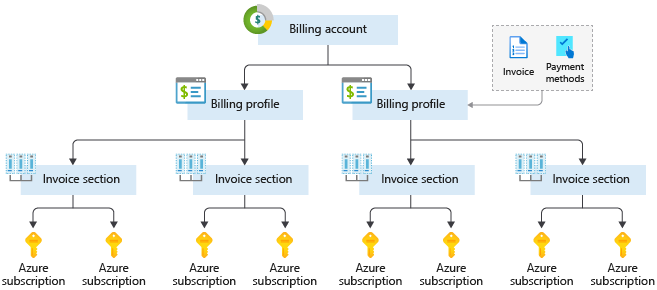
\includegraphics[width=15cm]{4-billing-structure-overview}
\end{center}
\section{Support options}
\subsection{Free resources}
\begin{itemize}
	\item Online documentation
	\item Community support
	\begin{itemize}
		\item Azure knowledge center
		\item Microsoft tech community
		\item Stack overflow
		\item Server fault
		\item Azure feedback forums
		\item Twitter
	\end{itemize}
	\item Demo videos
	\item Billing and subscription management support
	\item Azure quickstart center
	\item Azure service health
	\item Azure advisor
\end{itemize}
\subsection{Support plans}
{\renewcommand{\arraystretch}{2}
	\begin{tabularx}{\textwidth}{|L|L|L|L|}
		\hline
		& Developer & Standard & Professional Direct\\
		\hline
		Best for& Non-critical workloads&Production workloads & Business-critical workloads\\
		\hline
		Reactive technical support& 1 business day& 1 hour for critical& 1 hour and priority tracking for critical\\
		\hline
		Proactive technical support& N/A & N/A & Access to a pool of technical experts\\
		\hline
		
	\end{tabularx}
}

\end{document}
